\documentclass[margin=2pt]{standalone}
\usepackage[table]{xcolor}
\usepackage[utf8]{inputenc}
\usepackage[T1]{fontenc}

\usepackage{tikz}
\usepackage{helvet}
\usepackage{amsmath}

\usetikzlibrary{intersections, shapes.arrows, spath3, shapes.geometric, fit, backgrounds, calc, tikzmark, decorations.pathreplacing, angles, quotes}

\renewcommand\familydefault\sfdefault

% Use \phantom to hide text for exams
\renewcommand{\phantom}{}

\newcommand{\lOS}{\phantom{Operační}\\\phantom{systém}}
\newcommand{\lTask}{{úloha}}
\newcommand{\lTaskAddressSpace}{\phantom{adresový prostor}\\\phantom{úlohy}}
\newcommand{\lSection}{\phantom{Sekce}}
\newcommand{\lUnallocated}{\phantom{Nepřidělený}\\\phantom{prostor}}
\newcommand{\lFreeSpace}{\phantom{volná oblast}}

\newcommand{\memHeight}{100}
\newcommand{\memSize}{1024}
\newcommand{\memUnit}{K}

\definecolor{themeBlue}{RGB}{1, 103, 143}
\definecolor{themeOrange}{RGB}{221, 109, 16}
\definecolor{themeTeal}{RGB}{18, 54, 69}
\definecolor{themeGrey}{RGB}{120, 121, 124}

\newcommand{\memoryMaps}{%  
    {% Initials state
        os/312/\lOS/20,
        task/8/\lTask\space 1/4,
        free/32/\lFreeSpace /4,
        task/24/\lTask\space 4/4,   
        free/128/\lFreeSpace/4,
        task/128/\lTask\space 5/4,
        task/256/\lTask\space 6/4,
        free/136/\lFreeSpace/4
    },
    {% Memory shake-up
        os/312/\lOS/20,
        task/8/\lTask\space 1/4,
        task/24/\lTask\space 4/4,   
        task/128/\lTask\space 5/4,
        task/256/\lTask\space 6/4,
        free/296/\lFreeSpace/4
    },
    {% Task placed
        os/312/\lOS/20,
        task/8/\lTask\space 1/4,
        task/24/\lTask\space 4/4,   
        task/128/\lTask\space 5/4,
        task/256/\lTask\space 6/4,
        task/256/\lTask\space 7/4,
        free/40/\lFreeSpace/4
    },
}

\newcommand{\stateNames}{%
    {počáteční stav},
    {po provedeném\\zahušťování},
    {po přidělení sekce\\úloze 7},
}

\begin{document}
    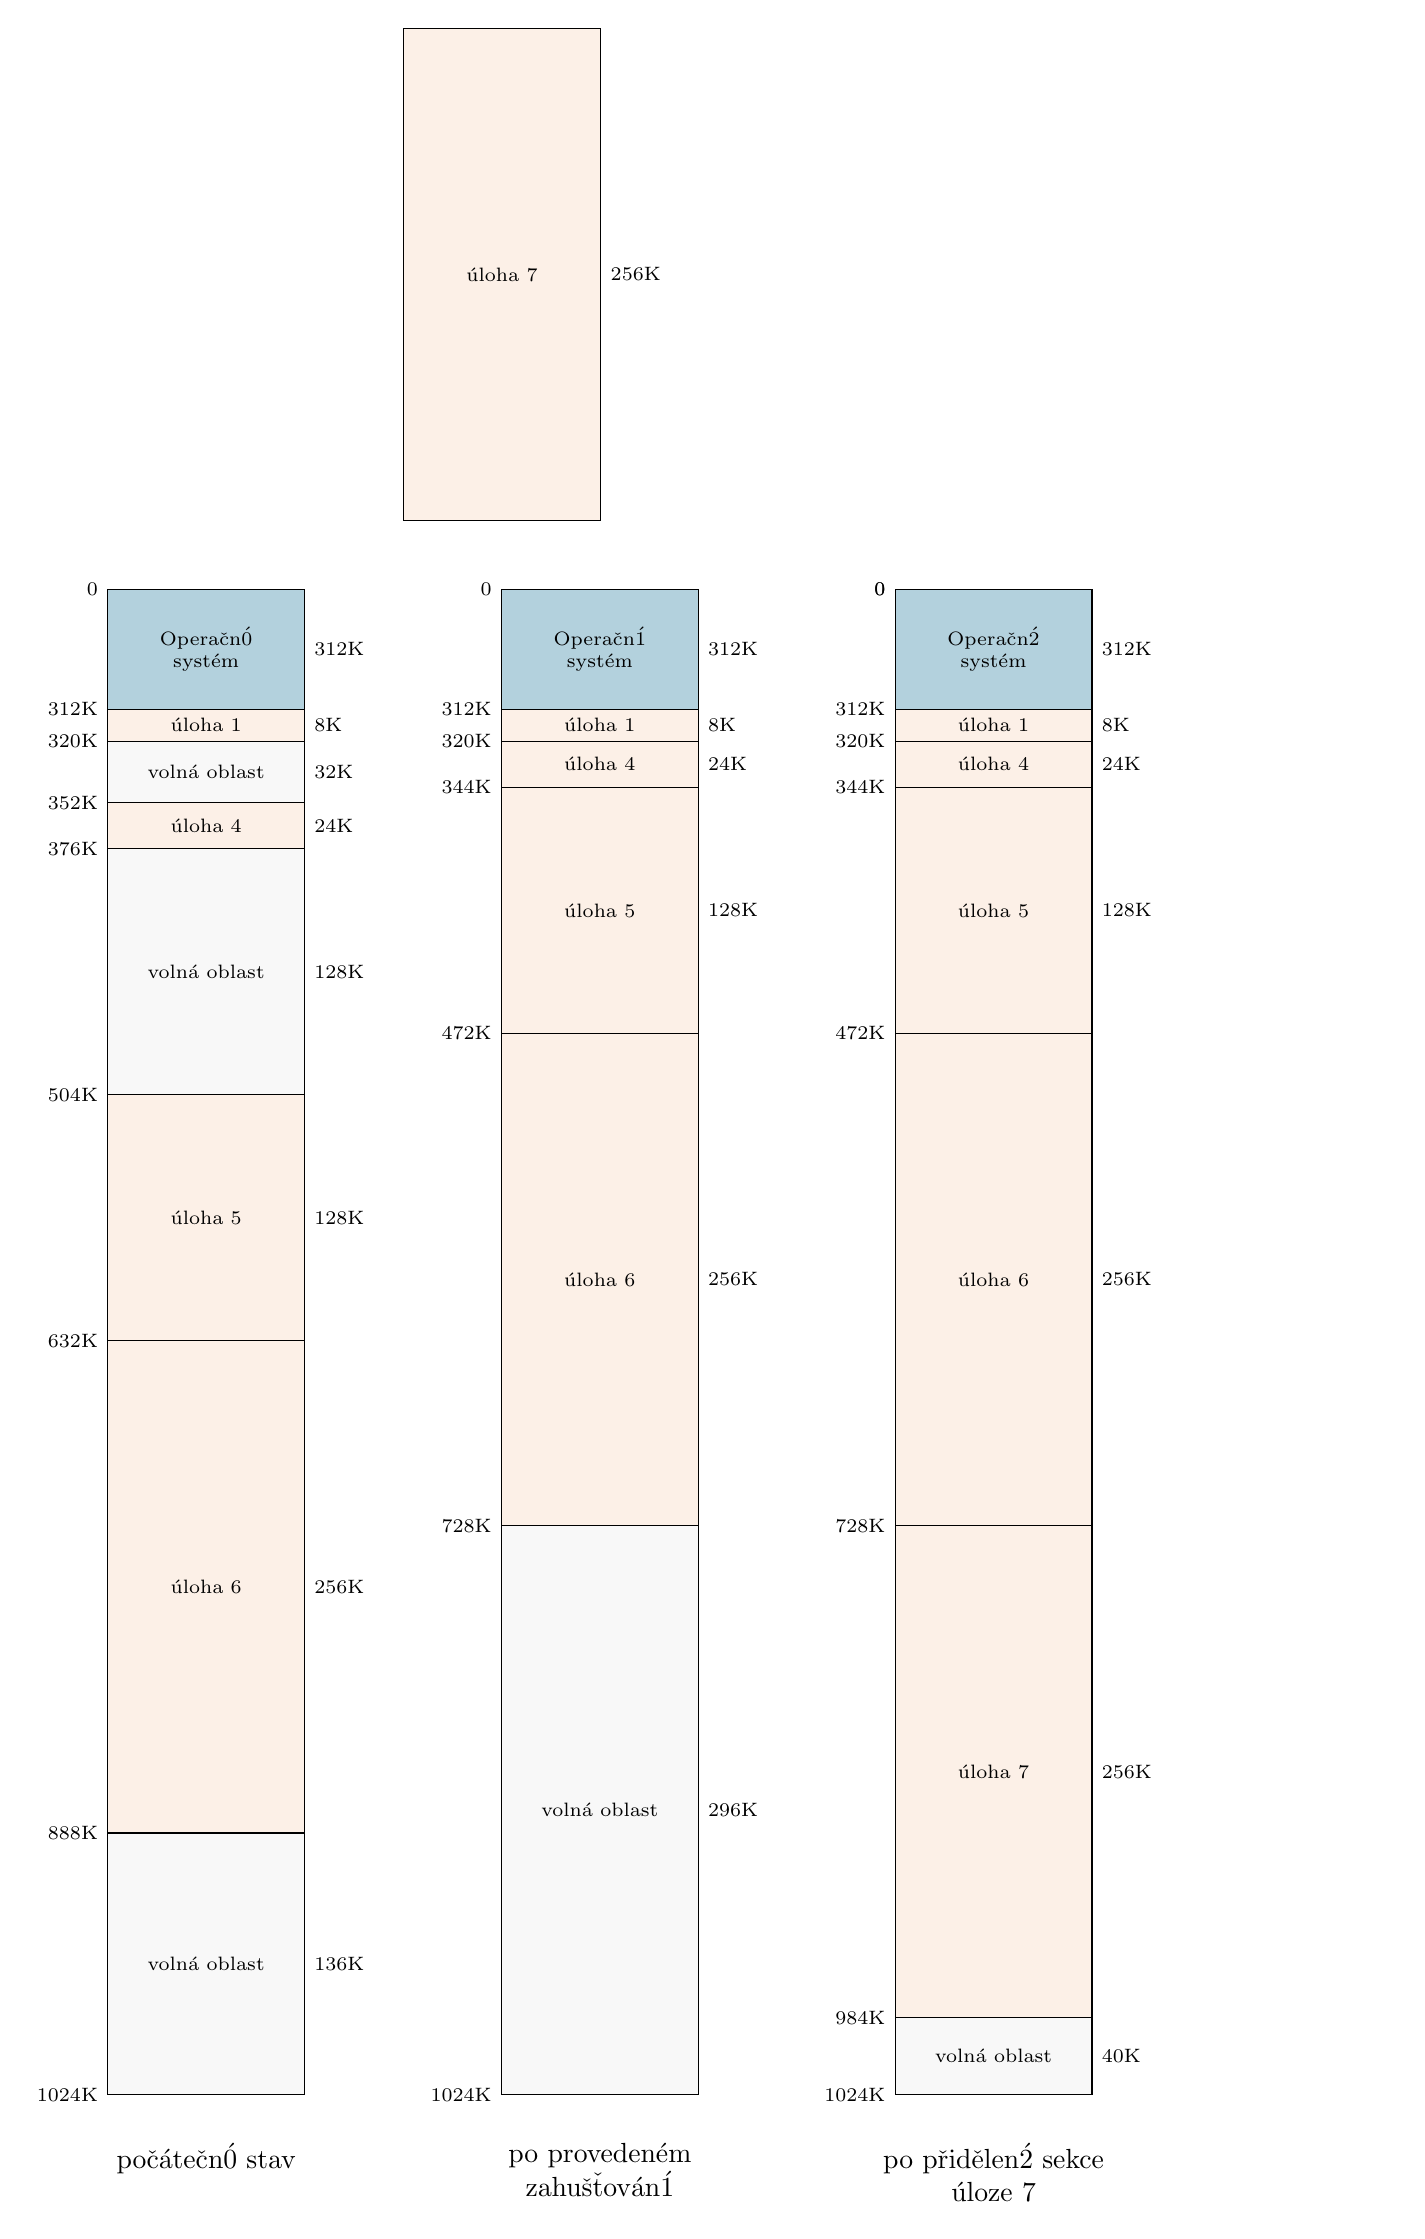
\begin{tikzpicture} [
        width/.style={minimum width=2.5cm},
        mem/.style={draw, width, anchor=north, align=center, minimum height=1.25cm, font=\scriptsize},
        label left/.style={font=\scriptsize, align=right, left},
        label right/.style={font=\scriptsize, right, align=left},
        brace mirror/.style={decoration={brace,mirror,raise=5pt}, decorate},
        brace/.style={decoration={brace,raise=5pt}, decorate},
        os/.style={fill=themeBlue!30},
        free/.style={fill=themeGrey!5},
        task/.style={fill=themeOrange!10},
    ]

    \foreach \map [expand list, count=\i from 0] in {\memoryMaps} {  
        \begin{scope}[xshift=5*\i cm]
            \coordinate (h0) at (0,0); % Hackish way to silence the first
            \xdef\memPosition{0}
      
            \foreach \type/\size/\label/\scale [expand list, count=\n from 1] in {\map} {
                \pgfmathsetmacro{\sectionUnit}{\memHeight/\memSize}
                \pgfmathsetmacro{\sectionSize}{(\sectionUnit * \size) /\scale}
                \pgfmathtruncatemacro{\lastn}{\n-1}
                
                \draw (h\lastn) node[mem, \type, anchor=north, outer sep=0, minimum height=\sectionSize cm] (sec \n) {\label};
                \draw (sec \n.east) node[label right] {\size\memUnit};
        
        
                \pgfmathparse{\memPosition + \size}
                \xdef\memPosition{\pgfmathresult}
                \pgfmathtruncatemacro{\pos}{\memPosition}
                \draw (sec \n.south west) node[label left] {\pos\memUnit};
                
                \coordinate (h\n) at (sec \n.south);
            }
            \draw (sec 1.north west) node[label left] {0};
        \end{scope}
    }

    \foreach \label [expand list, count=\i from 0] in {\stateNames} {
        \begin{scope}[xshift=5*\i cm]
            \coordinate (origin) at (0,0);
            \draw ($ (origin|-sec 7.south) - (0, .5) $) node[below, align=center] {\label};
        \end{scope}
    }

    \begin{scope}[shift={(2.5cm,4cm)}]
        \path let \p1=($(sec 6.north)-(sec 6.south)$)  
               in  node[mem, task, anchor=west,  minimum height=\y1] (new task) at (0,0)  {\lTask\space 7};
        \draw (new task.east) node[label right] {256\memUnit};
    \end{scope}
 
    \end{tikzpicture}
\end{document}